\subsection{Experimento 2 - Experiencias con osciloscopio de almacenamiento digital}

\vspace{5mm}
\subsubsection{Visualizando eventos no repetitivos – Barrido Único}

En este segundo experimento, se propone utilizar un osciloscopio digital con almacenamiento, en el modo de barrido. Este modo permite capturar eventos no repetitivos dentro de un circuito, por ejemplo, un fenómeno transitorio.

En este caso, el evento único que se analizará consistirá en un tren de pulsos producido por un sistema de discado telefónico rotativo (figura \ref{disco}). 

\begin{figure}[H]
    \centering
        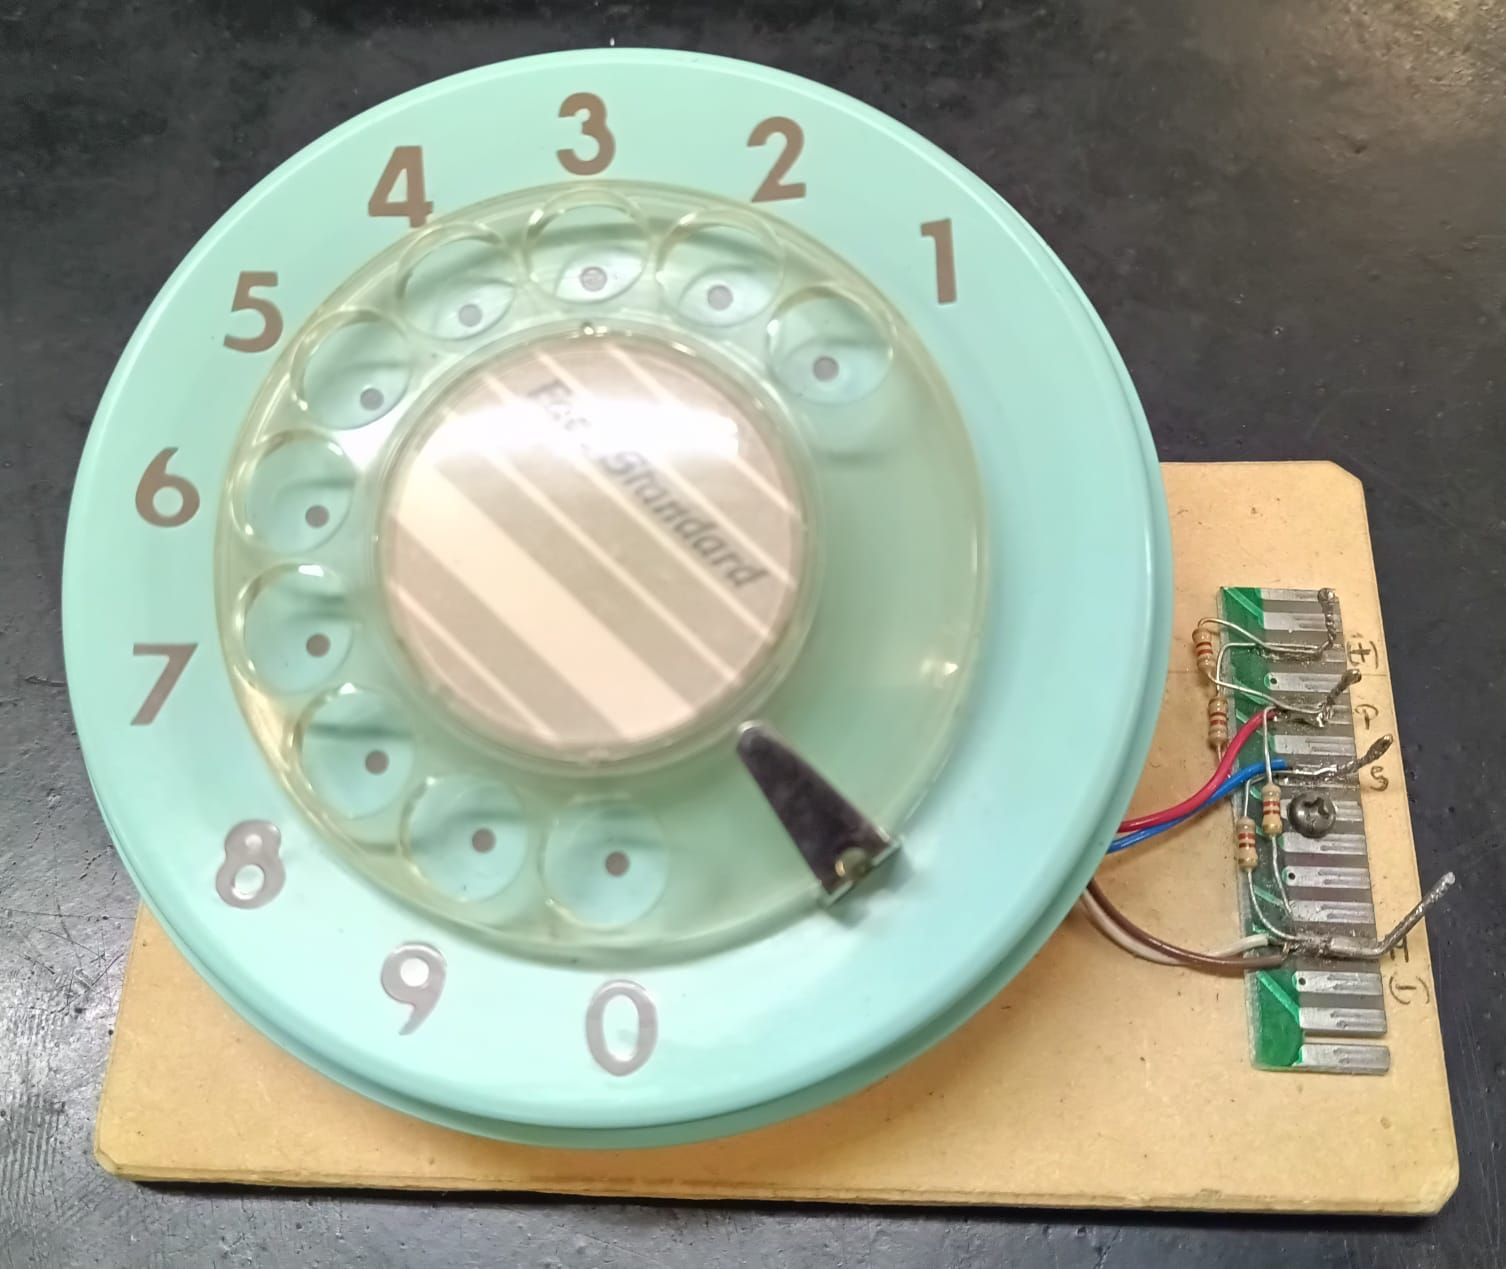
\includegraphics[width=0.5\textwidth]{Imagenes/discTel.jpeg}
    \caption{Kit generador de pulsos de disco telefónico}
    \label{disco}
\end{figure}

Este sistema de generación de pulsos consiste en un interruptor accionado mecánicamente mediante un disco rotativo que interrumpe la corriente de la línea tantas veces como el número que se está discando: Una vez para el número 1, cinco veces para el número 5, etc., a un ritmo cuyo valor nominal y óptimo debería ser 10 pulsos por segundo. Este tipo de discado se denomina “por desconexión del circuito”. 

El disco también posee un interruptor adicional cuya función es cortocircuitar el receptor del microteléfono para que los pulsos del discado no sean escuchados por la persona que llama. Este interruptor se cierra ni bien se acciona el disco, permanece en este estado durante la generación de los pulsos y se abre simultáneamente (o un poco después) de producido el último pulso de la secuencia. 
A continuación, se presenta una imagen con el circuito interno del kit provisto por la cátedra para esta experiencia y al lado,los pulsos que se esperan ver en cada salida (figura \ref{circTel}).

\begin{figure}[H]
    \centering
        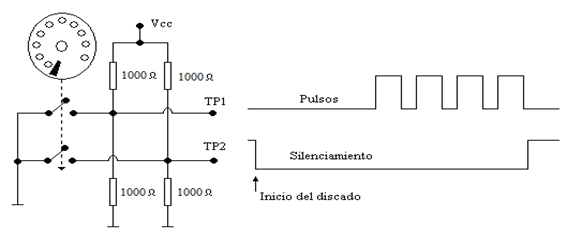
\includegraphics[width=\textwidth]{Imagenes/circTel.png}
    \caption{Circuito interno del kit y señales de salida}
    \label{circTel}
\end{figure}

Para este ensayo, se empleó en todas las instancias el osciloscopio digital \textit{RIGOL DS1052E}, con las siguientes configuraciones:

\begin{table}[H]
    \centering
    \scalebox{1}{
    \begin{tabular}{|c|c|c|c|c|c|c|}
    \hline
         V/div (Y1) & V/div (Y2) & t/div & Aten. Y1 & Aten. Y2 & Acop. & Barrido \\
    \hline
        2 $V$ & 2 $V$ & 100 $ms$ & x10 & x10 & CC & Único \\
    \hline
        \end{tabular}}
        \def\tablename{Tabla} 
        \caption{Cuadro de Controles}
        \label{tab:cont11}
\end{table}

El circuito del disco telefónico (figura \ref{circTel}) fue alimentado con una fuente de laboratorio de 12V de continua.



\vspace{10mm}
\textbf{Captura del tren de pulsos}

\vspace{3mm}
Para esta primera prueba, se seleccionó como fuente de disparo el canal uno (\textit{CH1}), el nivel de disparo en 2V, la pendiente en subida (\textit{slope} en +), y el inicio de disparo en 500ms (primera línea vertical desde la izquierda).

Luego de realizar los ajustes previamente descritos y conectar la punta al punto "\textit{TP1}" del circuito (figura \ref{circTel}), se procedió al experimento. Se pulsó el botón de "\textit{RUN/STOP}" del osciloscopio y se discó el número $8$ en el kit. El pulso detectado tuvo la siguiente forma (figura \ref{fig:disc8}):

\begin{figure}[H]
    \centering
        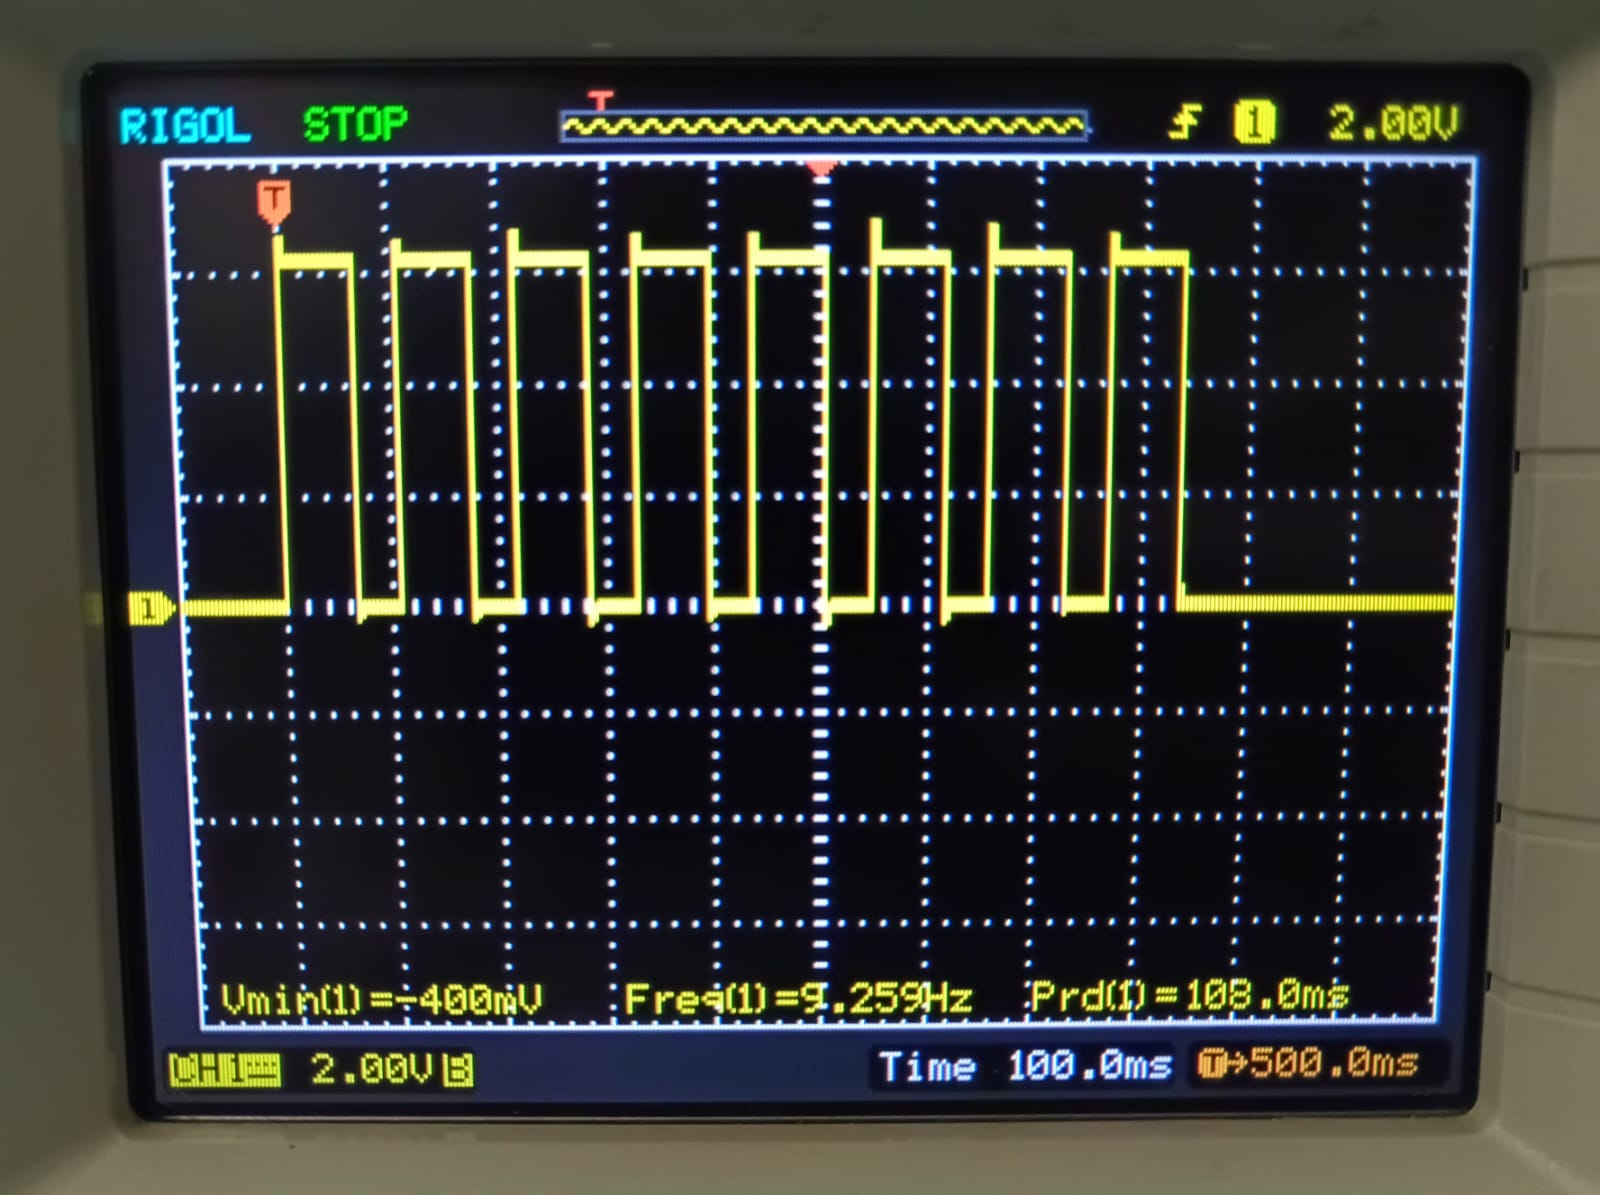
\includegraphics[width=0.7\textwidth]{Imagenes/tren8.jpeg}
    \caption{Tren de pulsos correspondientes al número $8$}
    \label{fig:disc8}
\end{figure}

En la imagen del osciloscopio se pueden apreciar claramente los ocho picos correspondientes al número elegido, por lo que el barrido fue exitoso y el circuito funciona como se esperaba.

También haciendo un poco de zoom, modificando la escala de tiempo se pueden visualizar la duración de los pulsos y los valles. 

\begin{table}[H]
    \centering
    \scalebox{1}{
    \begin{tabular}{c c | c}
         \multicolumn{3}{c}{Duración [ms]} \\
    \hline
         Pulsos & Valles & Periodo \\
         $t_p$ & $t_v$ & $T=t_{p}+t_{v}$   \\
    \hline
        68 & 40 & 108 \\
    \hline
        \end{tabular}}
        \def\tablename{Tabla} 
        \caption{Tiempos del tren de pulsos}
        \label{tab:durPul}
\end{table}

Para corroborar estas mediciones, se utilizó la función de medida del osciloscopio para medir el periodo de los pulsos. Este se puede ver en la esquina inferior derecha de la imagen en la figura \ref{fig:disc8}, con la leyenda "\textit{Prd(1)}", y coincide con el cálculo a partir de las lecturas. El periodo del tren de pulsos es de 108 ms, un valor muy cercano al ideal de 100 ms (expuesto antes como 10 pulsos por segundo). 

Como adicional, se midió el tren de pulsos para el número 0, y este fue el resultado (figura \ref{fig:disc0}). 

\begin{figure}[H]
    \centering
        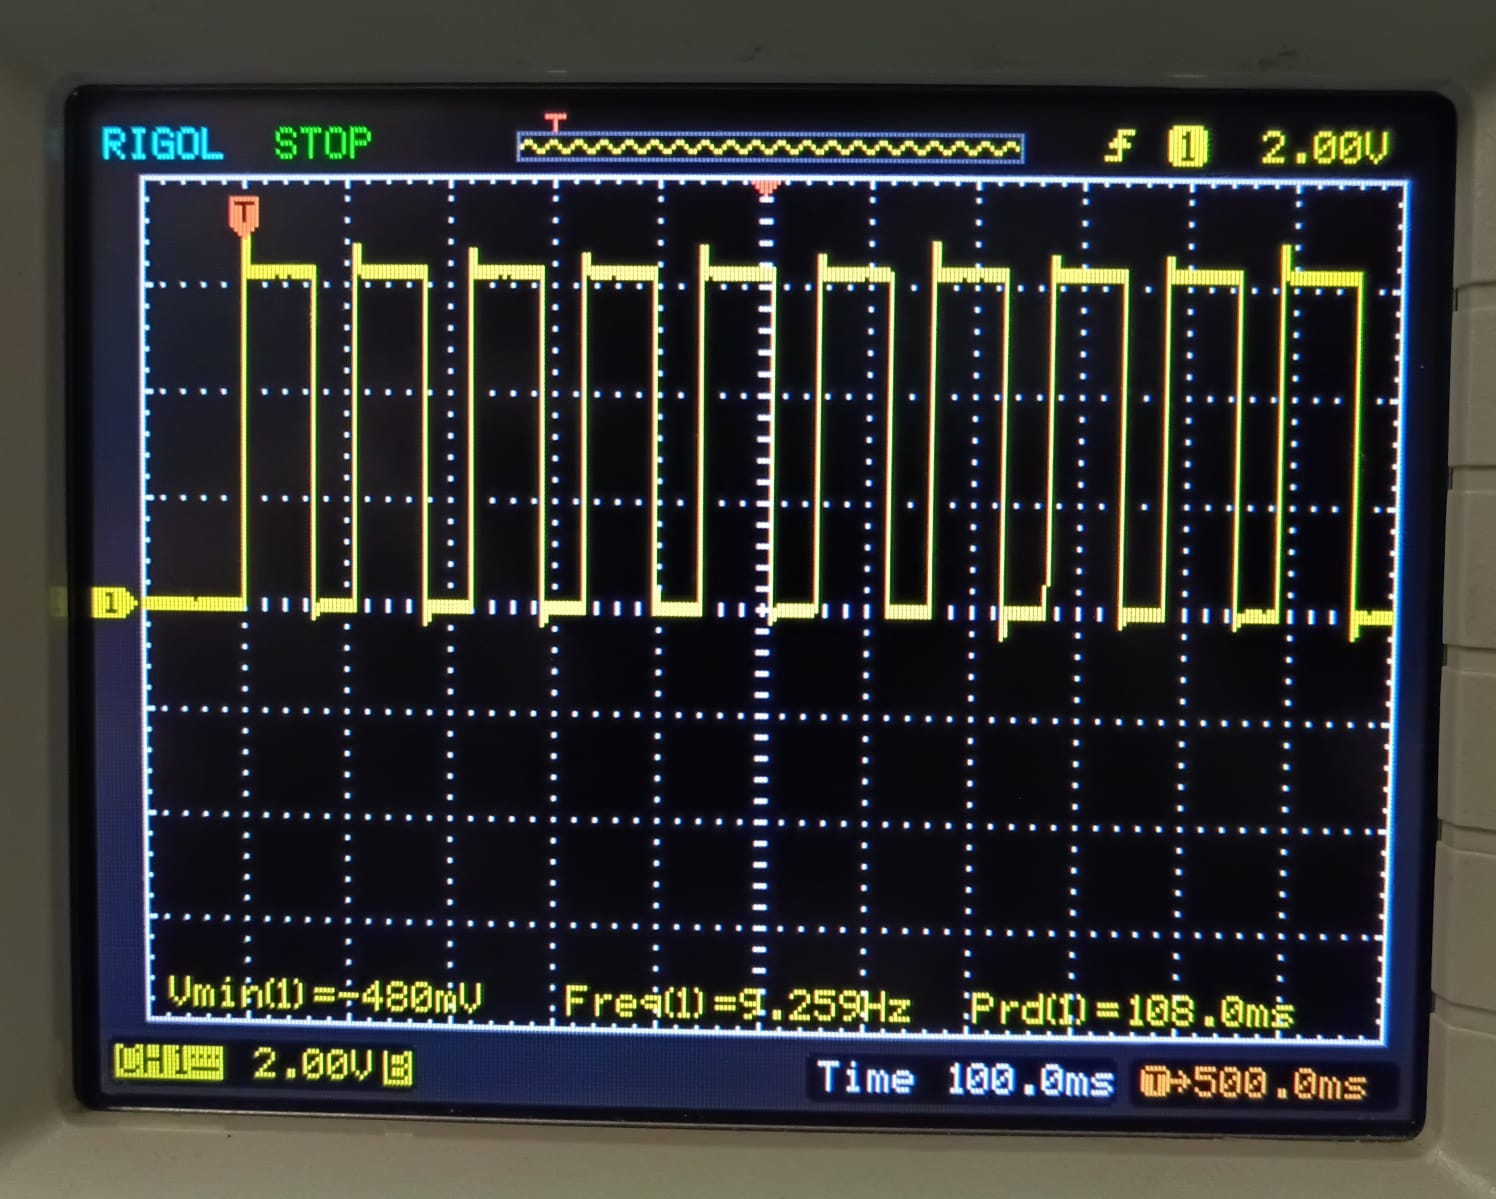
\includegraphics[width=0.7\textwidth]{Imagenes/tren0.jpeg}
    \caption{Tren de pulsos correspondientes al número $0$}
    \label{fig:disc0}
\end{figure}

Una cosa curiosa de esta lectura es que en lugar de verse cero pulsos como era de esperarse, hay diez. Luego pensándolo un poco, se llegó a la conclusión de que esto debe haberse diseñado así, para no ser confundido con el estado de inactividad. 



\vspace{10mm}
\textbf{Captura simultánea del tren de pulsos y de la señal de silenciamiento}
\vspace{3mm}

En esta última parte del trabajo se intentará capturar, simultáneamente, el tren de pulsos y la señal de silenciamiento.

Para esto, se cambió la fuente de disparo al canal dos (\textit{CH2}), la pendiente se puso en bajada (\textit{slope} en -) y el nivel de disparo en este canal en 2V. 

Una vez configurado el osciloscopio, se conectó la segunda punta (del canal 2) al punto "\textit{TP2}" del circuito (figura \ref{circTel}), y se discó el numero 3.

\begin{figure}[H]
    \centering
        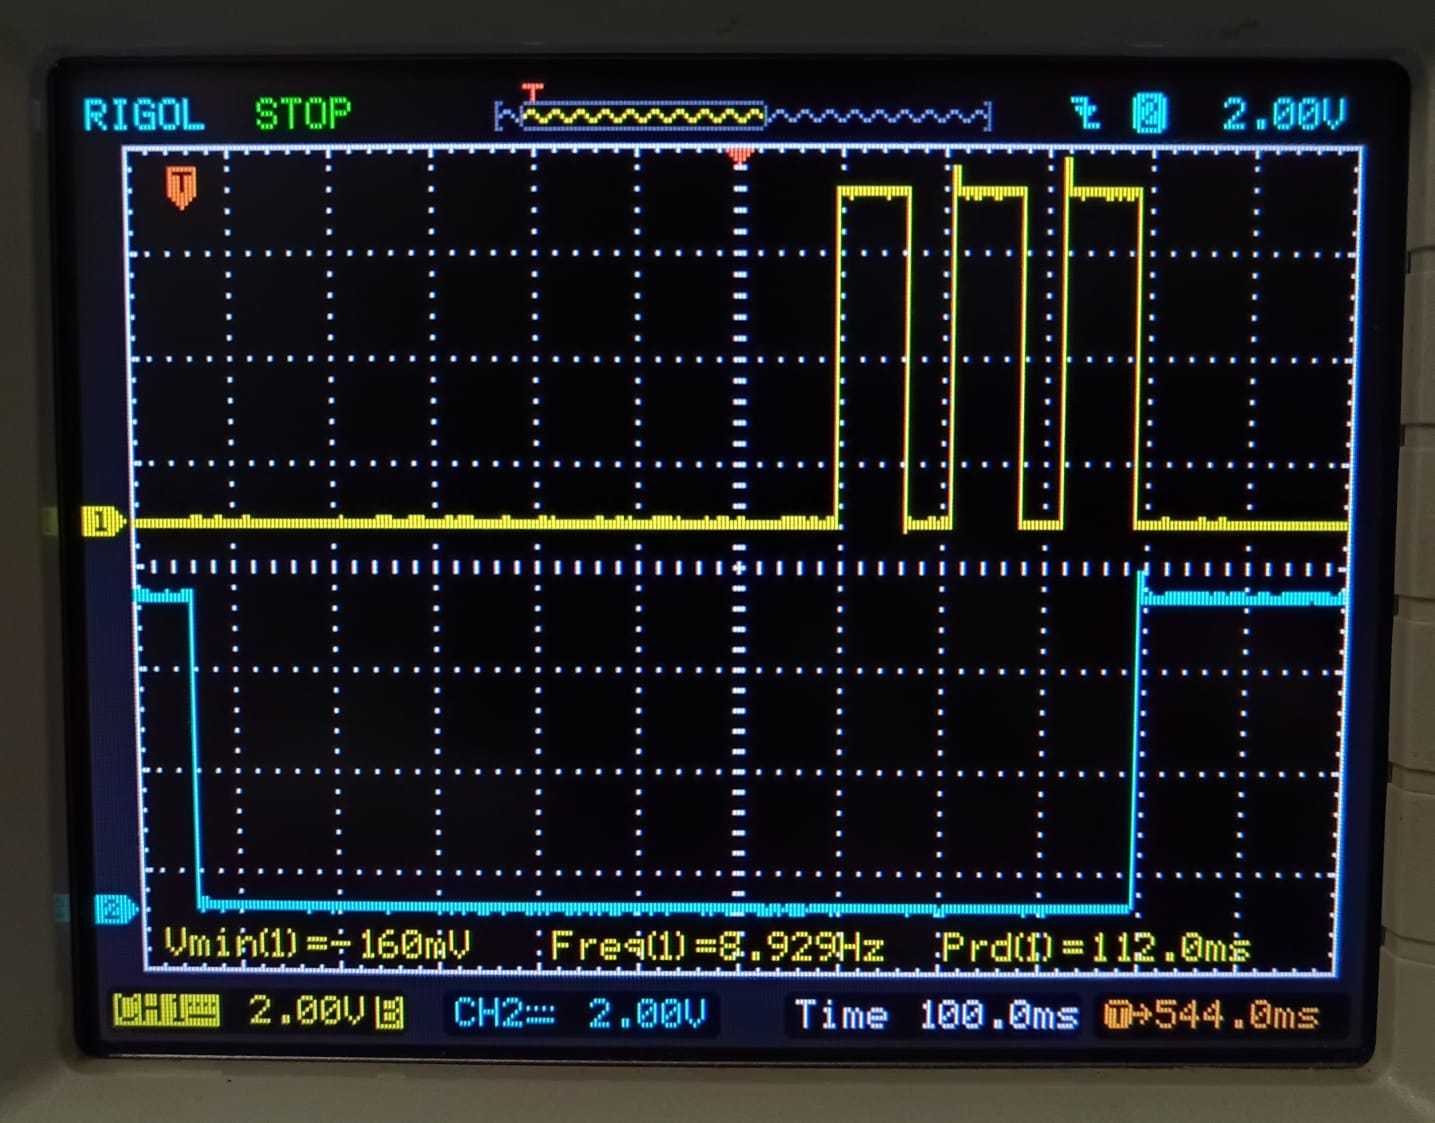
\includegraphics[width=0.6\textwidth]{Imagenes/tren3.jpeg}
    \caption{Tren de pulsos del número $3$ y señal de silenciamiento}
    \label{fig:disc3}
\end{figure}

En la figura \ref{fig:disc3}, abajo del tren de pulsos (señal amarilla), aparece otra señal que es la de silenciamiento (señal celeste). Efectivamente, esta señal se activa o se vuelve cero, apenas se acciona el circuito del disco, y recién se vuelve a un estado alto, cuando el mecanismo termina su recorrido y el tren de pulsos con el mensaje ha acabado. 

Idealmente este cambio al final del mensaje debería ser instantaneo, sin embargo aquí tenia cierto retardo. 

\begin{figure}[H]
    \centering
        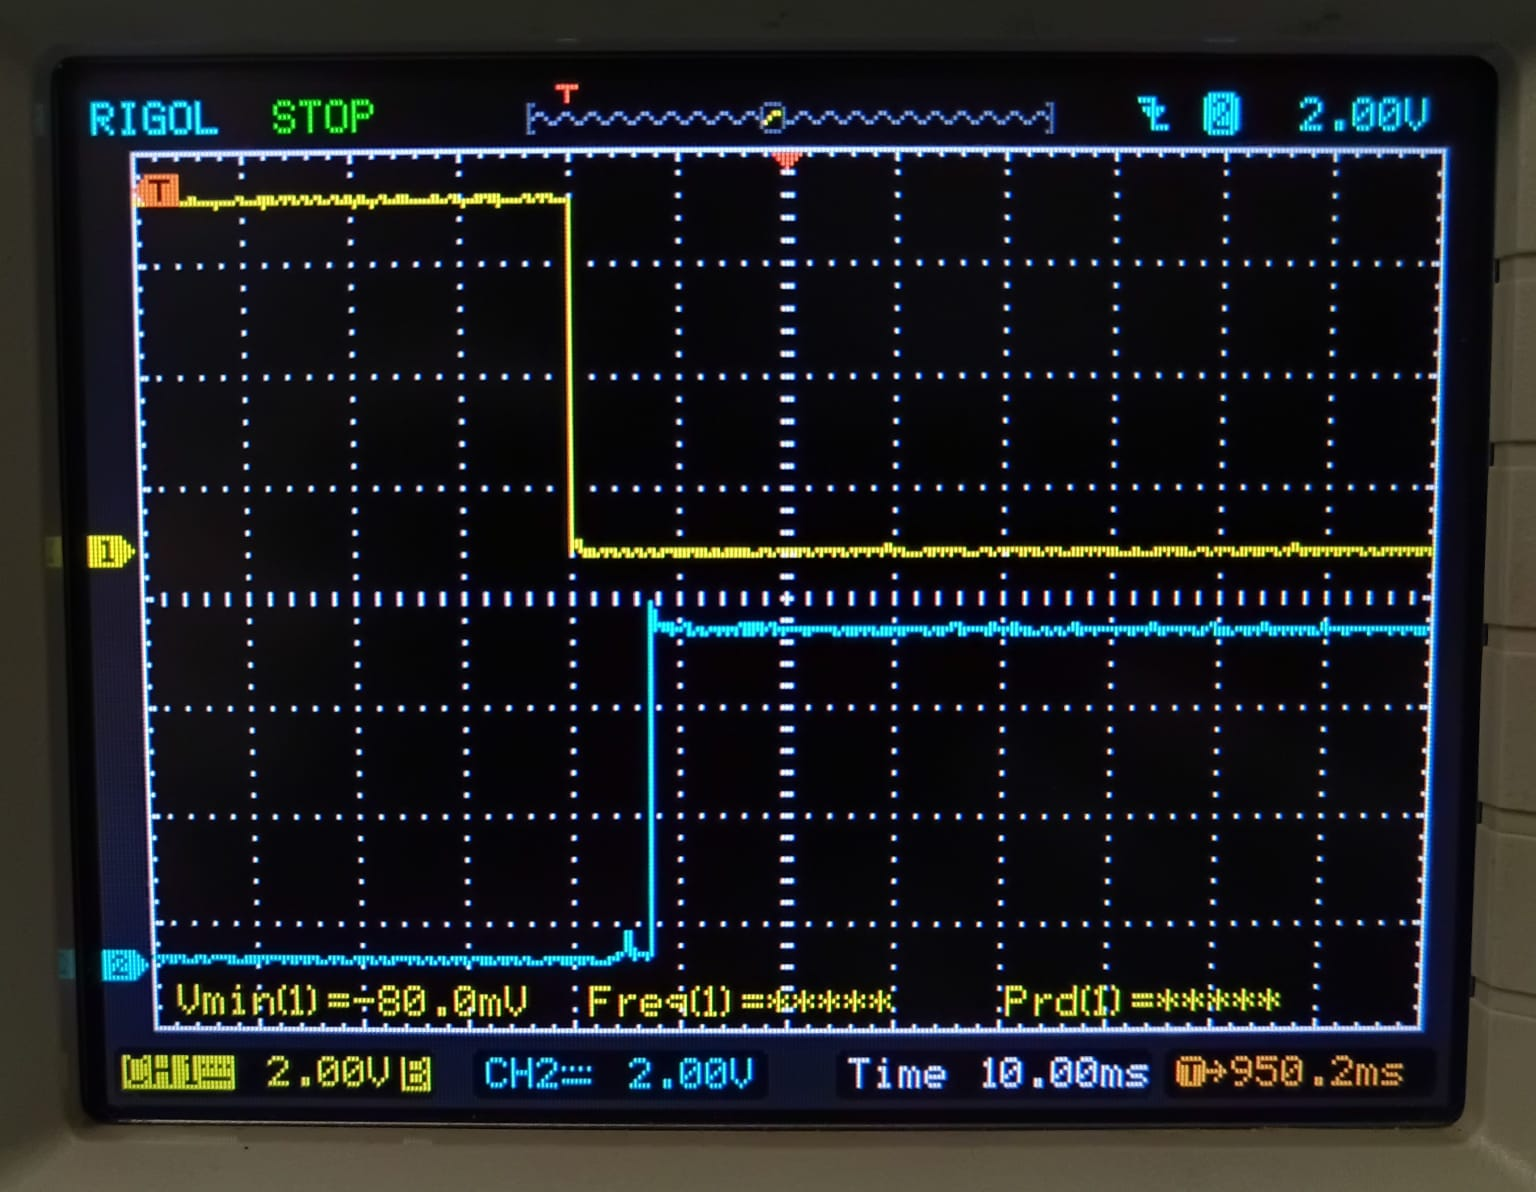
\includegraphics[width=0.6\textwidth]{Imagenes/delaySil.jpeg}
    \caption{Acercamiento al momento del final del mensaje y des-silenciamiento}
    \label{fig:delaySil}
\end{figure}

En el acercamiento al cambio de estado de la señal de silenciamiento, en la figura \ref{fig:delaySil}, se puede ver que el sistema tarda en desactivar la señal de silenciamiento, una vez finalizado el tren de pulsos.

En este caso el tiempo de demora $t_d$ es de aproximadamente \textbf{$7 ms$}. 


%Ver de añadir como adicional la figura del tren de nueve pulsos con la señal de silencio





